% !TEX root =  ../report.tex
% !TeX spellcheck = en-GB

\appendixpage
\setcounter{section}{0}
\renewcommand{\thesection}{\Alph{section}}

\section{Example CUDA program for vector addition}
\label{app:cudaEx}
\lstset{language=C, basicstyle=\linespread{1.1}\ttfamily\footnotesize,
frame=tlbr,
backgroundcolor=\color{lightgray!15},
showspaces=false, showstringspaces=false,
commentstyle=\ttfamily\footnotesize\color{gray},
escapechar=|,
emph={
       cudaMalloc, cudaFree,
       __global__, __shared__, __device__, __host__,
       __syncthreads,
   }
}
\lstinputlisting[language=C]{code/thread_add.cu}
\vspace{-1em}
\begin{adjustwidth}{-.5in}{-.5in}
\textbf{Compilation:}
\begin{verbatim}
> nvcc thread_add.cu -o thread_add
\end{verbatim}
\textbf{Result:}
\begin{footnotesize}
\begin{verbatim}
> ./thread_add
  03 06 07 05 03 05 06 02 09 01 02 07 00 09 03 06 00 06 02 06 01 08 07 09 02 00 02 03 07 05 09 02
  02 08 09 07 03 06 01 02 09 03 01 09 04 07 08 04 05 00 03 06 01 00 06 03 02 00 06 01 05 05 04 07

  05 14 16 12 06 11 07 04 18 04 03 16 04 16 11 10 05 06 05 12 02 08 13 12 04 00 08 04 12 10 13 09
\end{verbatim}
\end{footnotesize}
\end{adjustwidth}


\section{Getting Started with OP2}
\label{app:getStart}
The following is a guide for getting started with the \textit{airfoil} application, using the JIT compilation feature documented by this report.

\subsection{Source Code}
Firstly, the source code needs to be retrieved from GitHub, you can do using the following commands:
\begin{verbatim}
> git clone https://github.com/OP-DSL/OP2-Common.git
> cd OP2-Common/
> git checkout feature/jit
\end{verbatim}
This puts you in the feature branch for the project. \verb|git log| should give the latest commit as:
\begin{lstlisting}
commit 92865104e33e4448a180217a994b6cb1178bfab8
Author: NDunne <24ndunne24@gmail.com>
Date:   Fri May 8 12:51:08 2020 +0100

    Updated READMEs
\end{lstlisting}
If it does not, then more work may have been added to the branch, and the commit ID will be need to be checked out instead:
\begin{verbatim}
> git checkout 92865104e33e4448a180217a994b6cb1178bfab8
\end{verbatim}
This will leave you in a detached head state, but this is ok since we are just using the files, not modifying them for a future commit.
\clearpage
\noindent After obtaining the source code, check the contents of the current folder\\ (\verb|OP2-Common/|):
\begin{verbatim}
> ls
apps/  AUTHORS  cmake/  doc/  LICENSE  op2/  README  scripts/  translator/
\end{verbatim}
To double check that you do indeed have the JIT compilation feature, run the following command and confirm the result:
\begin{verbatim}
> ls translator/c/python/jit/
__init__.py  op2_gen_cuda_jit.py  op2_gen_seq_jit.py
\end{verbatim}

\subsection{System Setup}
As well as the OP2 source, we also require a number of dependency libraries, and need to set some environmental variables. I recommend adding these to a setup script, or to \verb|~/.bashrc| to save time in the future.

\subsubsection{3rd Party Libraries}
The OP2 framework relies on a couple of additional libraries:
\begin{itemize}
\begin{multicols}{2}
\item{C/C++ Compiler e.g.\ Intel \textit{icc}}
\item{HDF5}
\item{ParMetis}
\item{PT-SCOTCH}
\item{GNU Make}
\item{MPI Implementation e.g.\ Intel MPI}
\item{CUDA Toolkit}
\end{multicols}
\end{itemize}

\noindent If you are using a HPC cluster check if these are available using the \verb|module| command. If they are not, you will need to download and build each one.

\subsubsection{Environmental Variables}
Various Makefiles used by OP2 expect the below Environmental Variables to be set. An example \verb|~/.bashrc| script is show below, which gives example values for each.

\lstset{
   language=bash,
   keywordstyle=\color{teal}\textbf,
   stringstyle=\color{blue},
   identifierstyle=\itshape
}
\lstinputlisting{code/bashrc}

\noindent Once these have been set, you can compile the OP2 libraries and translate an application.
\clearpage
\subsubsection{OP2 Libraries}
With environmental variables set the next stage is to compile the OP2 library files. There is a different target for each hardware platform, but for this implementation the required targets are \verb|core|, \verb|cuda|, and \verb|hdf5|. Other back-ends are required for the tool to convert the input mesh to HDF5, so the command will just be \verb|make|, to build them all.
\begin{verbatim}
> cd op2/c/
> make
\end{verbatim}

\subsubsection{Airfoil}
The \textit{airfoil} source code can be found in the OP2 repository, by returning to the top level folder, and traversing to \verb|apps/c/airfoil/airfoil_JIT/dp/|.
\begin{verbatim}
> cd ../../
> cd apps/c/airfoil/airfoil_JIT/dp/
> ls
adt_calc.h  airfoil.cpp  bres_calc.h  convert_mesh.cpp  convert_mesh_mpi.cpp
Makefile  res_calc.h  save_soln.h  update.h
\end{verbatim}
The input data file will need to be downloaded from the OP2 Website into this directory, and as it is not already in the HDF5 data format, the \textit{convert\_mesh} tool will need to be built, and the file converted.
\begin{verbatim}
> wget https://op-dsl.github.io/docs/OP2/new_grid.dat
> make convert_mesh_seq
> ./convert_mesh_seq new_grid.dat
> mv new_grid_out.h5 new_grid.h5))
\end{verbatim}
Alternatively the MPI version can be used, by building the target \verb|convert_mesh_mpi|.
\par
The result will be a file \verb|new_grid.h5|. You can view the contents using \verb|h5dump|.

\tinytitle{Code Generation}

\noindent It is time to perform the code generation step. As in seen in Section \ref{ss:results}, the command is as follows, as long as the \verb|$OP2_INSTALL_PATH| environmental variable is correctly configured.
\begin{verbatim}
> python2 $OP2_INSTALL_PATH/../translator/c/python/op2.py airfoil.cpp JIT
> ls
adt_calc.h      bres_calc.h     convert_mesh_seq     new_grid.dat
save_soln.h     airfoil.cpp     convert_mesh.cpp     cuda/
new_grid.h5     seq/            airfoil_op.cpp       convert_mesh_mpi.cpp
Makefile        res_calc.h      update.h
\end{verbatim}
The generated code is now present, and can be seen in the folder named \verb|cuda/|. It is ready to be compiled into an executable.

\tinytitle{Compilation}

\noindent Using the Makefile to compile, both a JIT enabled and disabled binary can be produced easily. For JIT compilation enabled:
\begin{verbatim}
> make airfoil_cuda
> ./airfoil_cuda_jit
\end{verbatim}
And for disabled:
\begin{verbatim}
> make airfoil_cuda JIT=FALSE
> ./airfoil_cuda
\end{verbatim}

\noindent And the binaries should run as expected, and pass the test after 1000 iterations.

\subsection{Other Applications}
The translator script should work just as well with other applications written for OP2, however they will need to reproduce the Makefile in order to work correctly. It is required that the Makefile is accessible by the running application for JIT compilation to work correctly, and must contain a target similar to the following:
% \makebox[\textwidth][c]{

\begin{lstlisting}[frame=none, backgroundcolor=\color{white}, language=bash]
airfoil_cuda_rec: jit_const.h
  nvcc $(VAR) $(INC) $(NVCCFLAGS) $(NVCC_COPTS) $(OP2_INC) -Icuda -I. -c \
  ./cuda/adt_calc_kernel_rec.cu -o ./cuda/adt_calc_kernel_rec.o
  nvcc $(VAR) $(INC) $(NVCCFLAGS) $(NVCC_COPTS) $(OP2_INC) -Icuda -I. -c \
  ./cuda/bres_calc_kernel_rec.cu -o ./cuda/bres_calc_kernel_rec.o
  nvcc $(VAR) $(INC) $(NVCCFLAGS) $(NVCC_COPTS) $(OP2_INC) -Icuda -I. -c \
  ./cuda/res_calc_kernel_rec.cu -o ./cuda/res_calc_kernel_rec.o
  nvcc $(VAR) $(INC) $(NVCCFLAGS) $(NVCC_COPTS) $(OP2_INC) -Icuda -I. -c \
  ./cuda/save_soln_kernel_rec.cu -o ./cuda/save_soln_kernel_rec.o
  nvcc $(VAR) $(INC) $(NVCCFLAGS) $(NVCC_COPTS) $(OP2_INC) -Icuda -I. -c \
  ./cuda/update_kernel_rec.cu -o ./cuda/update_kernel_rec.o   \
  nvcc cuda/adt_calc_kernel_rec.o cuda/bres_calc_kernel_rec.o \
  cuda/res_calc_kernel_rec.o cuda/save_soln_kernel_rec.o      \
  ccuda/update_kernel_rec.o -shared -o ./cuda/airfoil_kernel_rec.so
\end{lstlisting}

% }
\noindent The target compiles each of the JIT kernel files into an object file, then combines all the objects into a single Shared Object called \verb|cuda/airfoil_kernel_rec.so|. The name of the resultant DLL must follow this name pattern, otherwise it will not be found by the JIT enabled binary.

\clearpage
\section{Time Investment}
\label{app:tracker}
\begin{figure}[h]
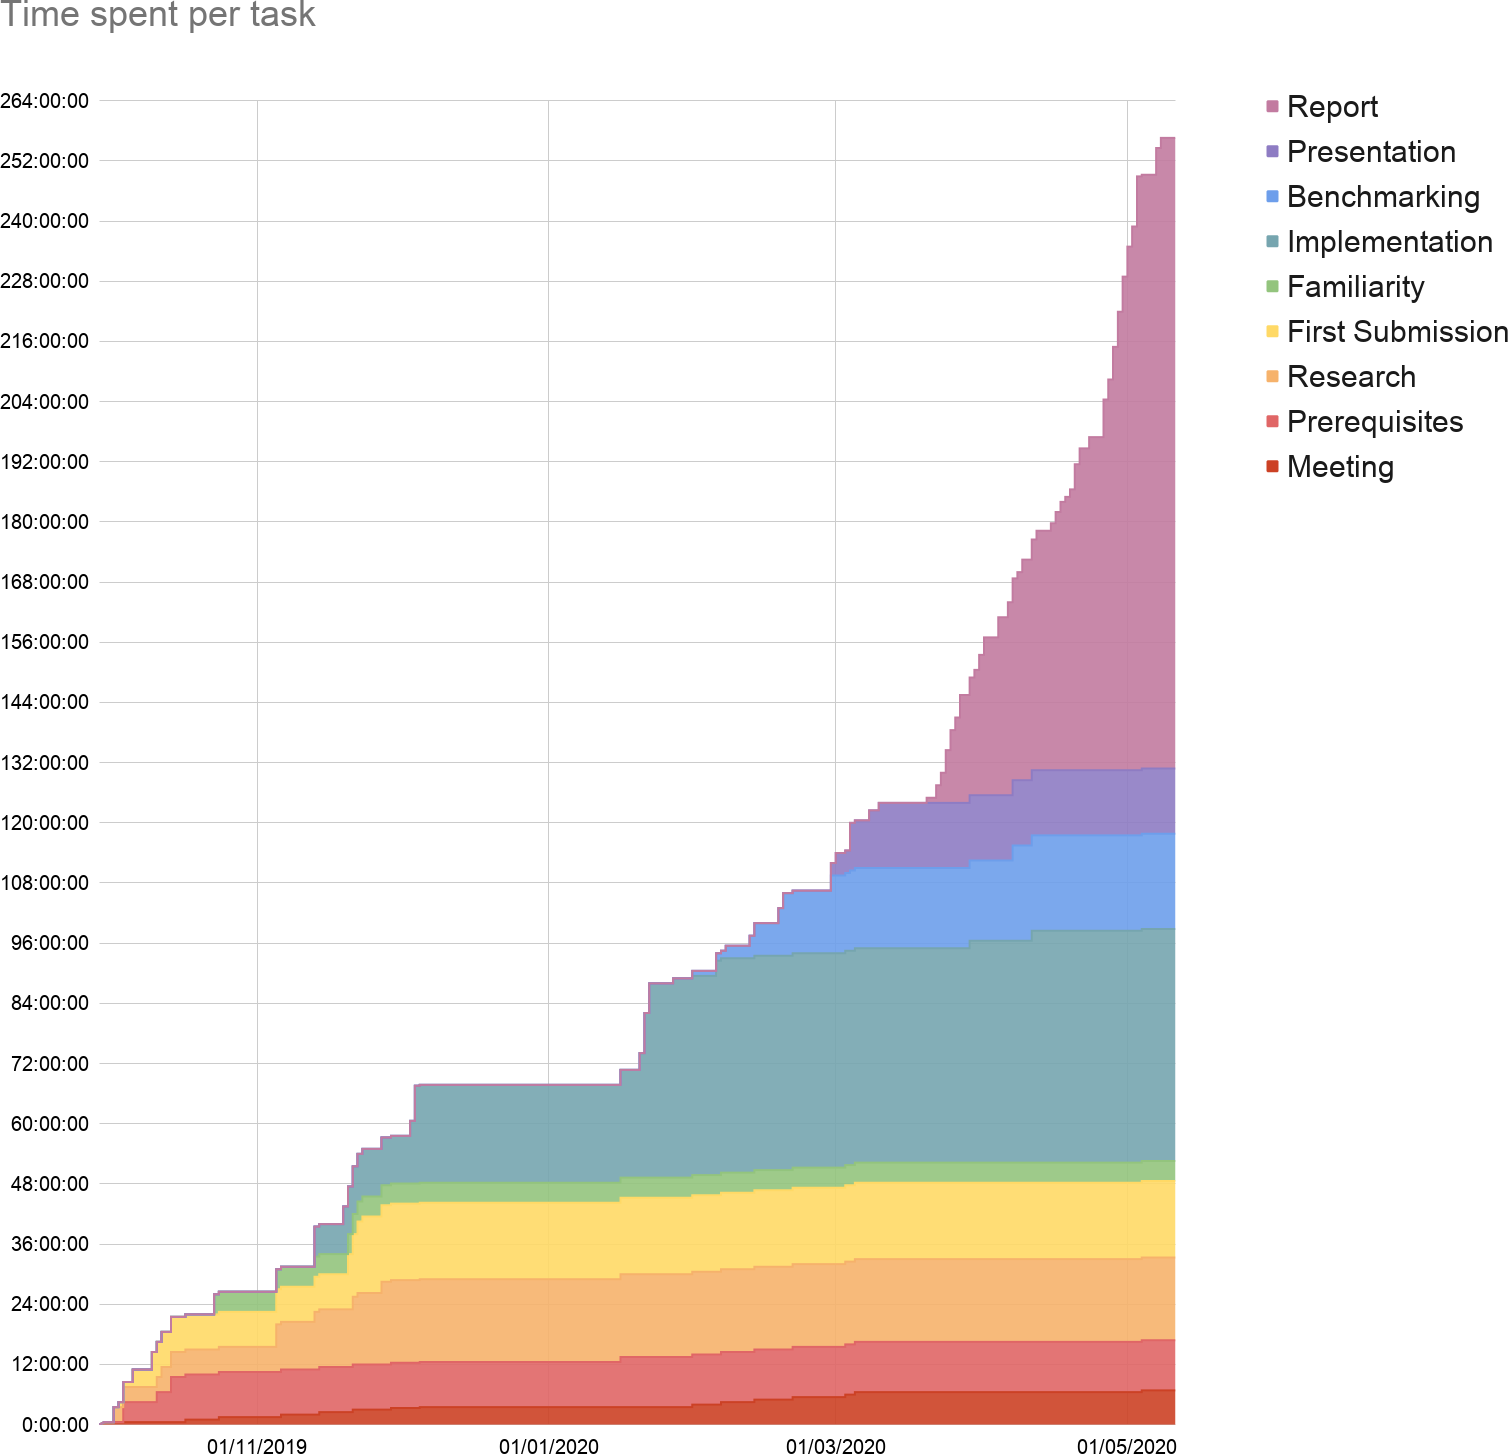
\includegraphics[width=\textwidth]{tracker}
\caption{\label{fig:tracker}Time Investment broken down by task.}

\vspace{1em}
While working on this project I attempted to track all the time I put into it, in an attempt to hold myself accountable and ensure work was done at a reasonable rate. The result is the graph above, plotted stacked to track total time investment also.
\end{figure}
